After learning our separate posteriors and clustering $\gvn$, along with the weather thresholds used in $\fvn$, we can now analyze and apply our results to our original goals of understanding and generating failure conditions.

\subsection{Analyzing Learned Posteriors}

For our two user-defined parameters, we choose $\xth=15$ minutes for our delay threshold and $\yth=72$ operations per hour for our demand threshold in $\gvn$. For both $\fvn$ and $\gvn$, we use $\alpha=50$ as the boundary sharpness scaling parameter. Although LGA is currently supposed to have hourly limits of 71 for scheduled operations and 3 for unscheduled operations during slot-controlled hours, historical practices still allow for scheduled operations to be between 72 and 75 in most hours \cite{faa_lga_2024}. The final results of the learned parameters are
% \begin{align}
%     \wthvf&=1.392,\qquad
%     \wthcf=1318,\qquad\\
%     \wthvg&=1.600,\qquad
%     \wthcg=1276,
% \end{align}
\begin{table}[htb!]
    \centering
    \begin{tabular}{|c||c|c||c|c|}
        \hline
        Parameter & Value & Units & Type & Function\\
        \hline\hline
        $\wthvf$ & $1.392$ & miles & visibility & $\fvn$ \\
        \hline
        $\wthvg$ & $1.600$ & miles & visibility & $\gvn$ \\
        \hline\hline
        $\wthcf$ & $1318$ & feet & ceiling & $\fvn$ \\
        \hline
        $\wthcg$ & $1276$ & feet & ceiling & $\gvn$ \\
        \hline
    \end{tabular}
    \caption{Final learned visibility and ceiling thresholds}
    \label{tab:learned-thresholds}
\end{table}

where $\wthvf$ and $\wthvg$ are in statute miles and $\wthcf$ and $\wthcg$ are in feet. Our final ELBO loss, i.e. negated ELBO, was $-204.34$ nats/dim. \cref{fig:q-phi-combined} shows the posterior distributions for the learned mean service times constructed from $10000$ samples for each cluster determined by $d= \gvd{x,y,w}$, for each of the eight labels $d\in \{0,1\}^3$, and \cref{tab:q-phi-results} displays some summary statistics. We can see that the posteriors appear to be reasonable, because the more nominal posteriors are near $0.0125$ hours, a mean service time which corresponds to a realistic capacity of $80$ operations per hour for LGA.

\begin{figure}[htb!]
    \centering
    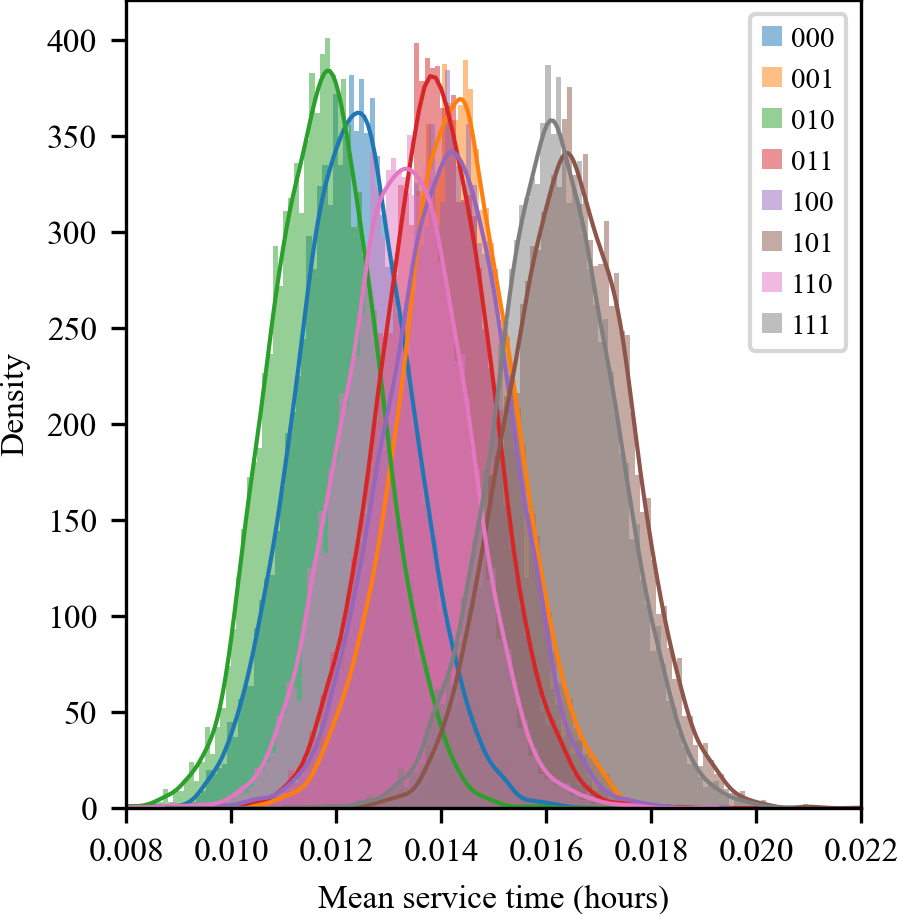
\includegraphics[height=3.0in]{media/q_phi_nsf_730_all.png}
    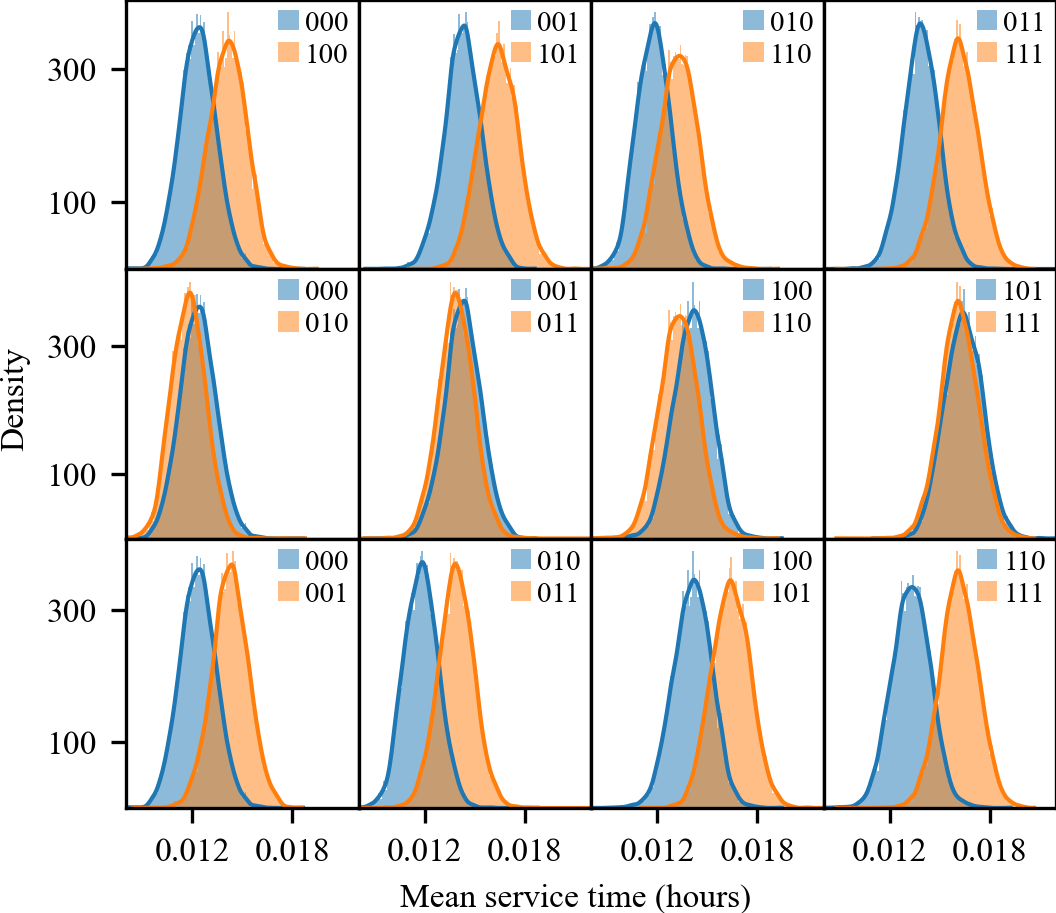
\includegraphics[height=3.0in]{media/q_phi_nsf_730_grid.png}
    \caption{Variational approximations for the mean service time $\rz$, for eight cluster labels $d\in\{0,1\}^3$. On the left, we plot the posteriors for all eight clusters for comparison. On the right, we plot pairs where two components of the label are held constant for each value in $\{0,1\}^2$ across the row, and the third is varied between $\{0,1\}$, with $d_x$, $d_y$, and $d_w$ being varied in the first, second, and third rows, respectively.}
    \label{fig:q-phi-combined}
\end{figure}

% 000 posterior, mean=0.01234, std=0.00110
% 001 posterior, mean=0.01429, std=0.00111
% 010 posterior, mean=0.01178, std=0.00104
% 011 posterior, mean=0.01389, std=0.00109
% 100 posterior, mean=0.01411, std=0.00116
% 101 posterior, mean=0.01643, std=0.00116
% 110 posterior, mean=0.01329, std=0.00117
% 111 posterior, mean=0.01617, std=0.00115

\begin{table}[htb]
    \centering
    \begin{tabular}{|c|c|c||c|c|}
        \hline
        $d_x$ & $d_y$ & $d_w$ & $\hat\mu$ (hrs) & $\hat\sigma$ (hrs) \\
        \hline\hline
        0 & 0 & 0 & 0.01234 & 0.00110 \\
        \hline
        0 & 0 & 1 & 0.01429 & 0.00111 \\
        \hline
        0 & 1 & 0 & 0.01178 & 0.00104 \\
        \hline
        0 & 1 & 1 & 0.01389 & 0.00109 \\
        \hline
        1 & 0 & 0 & 0.01411 & 0.00116 \\
        \hline
        1 & 0 & 1 & 0.01643 & 0.00116 \\
        \hline
        1 & 1 & 0 & 0.01329 & 0.00117 \\
        \hline
        1 & 1 & 1 & 0.01617 & 0.00115 \\
        \hline
    \end{tabular}
    \caption{Estimated mean $\hat\mu$ and standard deviation $\hat\sigma$ in hours for learned posteriors $\qvn$.}
    \label{tab:q-phi-results}
\end{table}

Using the pairwise comparison plots in the grid on the right side of \cref{fig:q-phi-combined}, we can investigate the effect of each component of $d$ on the learned posterior for its cluster. In the first row, where only $d_x$ is varied in each plot, we note that the posteriors for $d_x=0$ (blue) are to the left of those for $d_x=1$ (orange). This shows that introducing more delays corresponds to shifting the learned posterior to the right, which is what we expected to see. Similarly, in the third row, where only $d_w$ is varied in each plot, we note that the posteriors for $d_w=0$ (blue) are to the left of those for $d_w=1$ (orange), which also aligns with the belief that worse weather leads to higher service times that we incorporated into the model.

In the second row, where only $d_y$ is varied in each plot, we observe a slightly different effect, although it is a bit less evident. Here, the posteriors for $d_y=0$ (blue) appear to be shifted to the right, in comparison to $d_y=1$ (orange). However, this still makes sense, because it is showing the effect of scheduled demand on delay that we had previously discovered in \cref{sec:atrds-single-airport}, that because of the higher scheduled demand, a lower mean service time may be required to achieve the same performance in terms of delays on a busier day versus a lighter one, all else held equal, which manifests here as the posterior for that particular cluster being shifted to the left slightly.


\subsection{Using Learned Posteriors}

Now that we have learned posteriors for our separate clusters, we can use them in our learned generative model, and analyze the results, similar to sampling from the posterior predictive distribution after learning an approximation for the posterior. 

\begin{figure}[htb!]
    \centering
    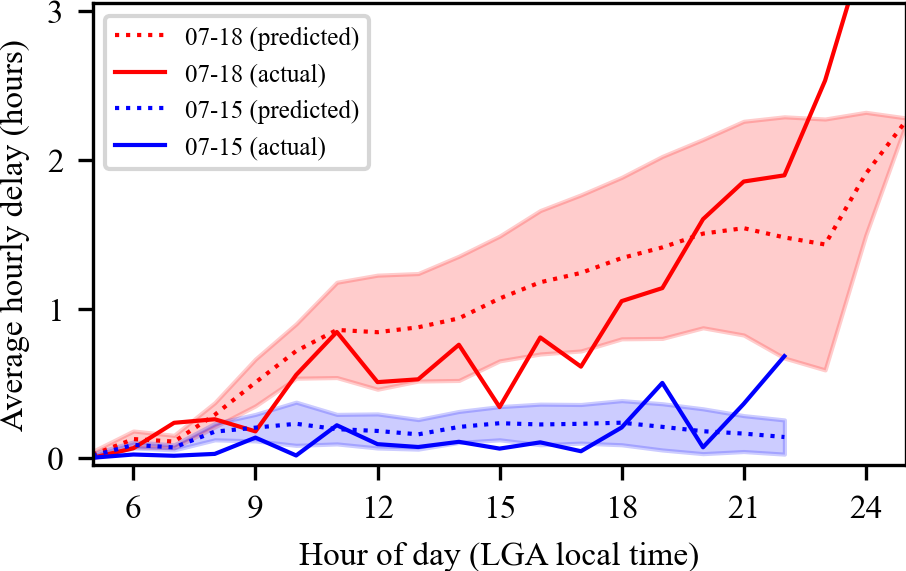
\includegraphics[width=0.7\linewidth]{media/posterior_predictive_comparison.png}
    \caption{Actual and predicted mean hourly delays using our model, with a weather-induced delay applied on one day (red) and nominal operations on the other (blue).}
    \label{fig:pp-comparison}
\end{figure}

We first select two days for analysis, which are July 18, 2019 (day 1) and July 15, 2019 (day 2). For both days, the peak scheduled hourly demand is $75$ operations, which is above $\yth$, so $d_{y,1}=d_{y,2}=1$. Additionally, the weather values for each day are $w_1=(10.0, 8649.3)$ and $w_2=(2.414,299.2)$, so $d_{w,1}\approx 0$ and $d_{w,2}\approx 1$. In reality, day 1 (red) has high delays above $\xth$, while day 2 (blue) does not, as seen in the solid lines in \cref{fig:pp-comparison}, so for comparison, we also select $d_{x,1}=1$ and $d_{x,2}=0$. Then, using each of these posteriors corresponding to $d_1$ and $d_2$ in the model, we can generate predictive samples, shown in the dotted lines and shaded regions in the figure. These are consistent with the actual outcomes, which shows that our learned generative model is able to accurately take in conditions of interest and generate a realistic result of imposing them onto a given day, showing its value as a predictive tool. The key here is that we can take $y$ and $w$ for a new day, which we would know from a schedule and forecast, respectively, and come up with distributions for $z$ that should lead to a desired level of delay, and doing so does appear to match what actually happens.

\begin{figure}[htb!]
    \centering
    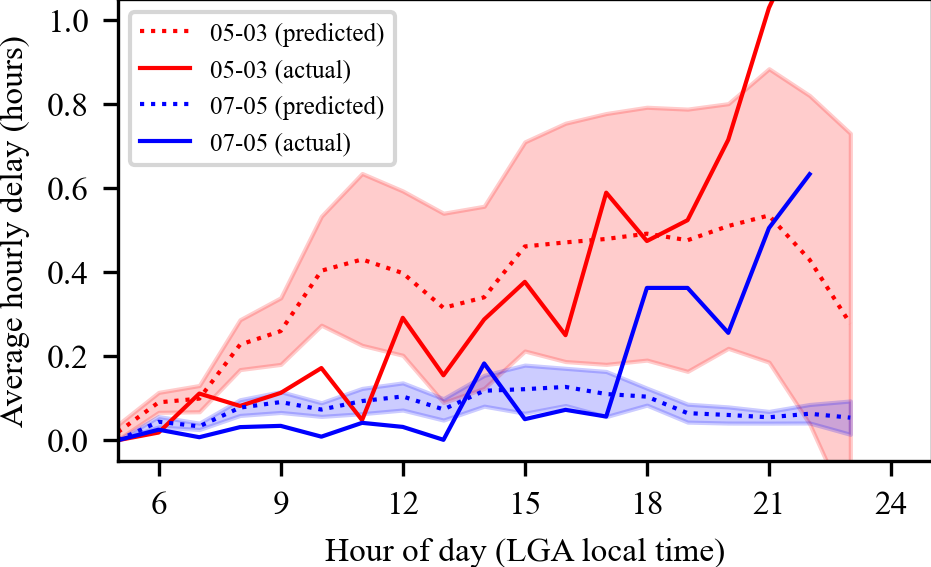
\includegraphics[width=0.7\linewidth]{media/posterior_predictive_comparison_alt.png}
    \caption{Actual and predicted mean hourly delays using our model, with a demand-induced delay applied on one day (red) and nominal operations on the other (blue).}
    \label{fig:pp-comparison-alt}
\end{figure}

% Actual vs predicted hourly delay using our model for two days, the plot in red shown for a day with weather-induced delay that our model successfully replicates (predicted average and standard deviation for 20 samples shown in the plots). The plot in blue shows hourly delays for a day with observed delays to be less than 15 minutes.

Similarly, we examine another pair of days, May 3, 2019 (day 1) and July 5, 2019 (day 2). This time, we have $w_1=(1.609,162.7)$ and $w_2=(10.0,574.9)$, so $d_{w,1}\approx d_{w,2}\approx 1$. However, this time we have $y_1$ above the threshold $\yth$ and $y_2$ below it, so $d_{y,1}=1$ and $d_{y,1}=0$. Similarly to before, we follow the actual observation for comparison, so we use $d_{x,1}=1$ and $d_{x,2}=0$. We visualize this in \cref{fig:pp-comparison-alt}, where we can see the effect of varying the imposed demand in our generative model, and that it also resembles reality for the two day in question.

In these two case studies, we have seen that our learned model and posteriors, although somewhat coarse, do appear to be capable of generating useful and realistic results. Because of the simplified model, we can simply sample adversarial weather conditions by using the learned thresholds, but we will leave investigating more complex structures as part of the plan for future work.